\documentclass[10pt]{beamer}

\usetheme[progressbar=frametitle]{metropolis}
\usepackage{appendixnumberbeamer}
\usepackage{graphicx}
\usepackage{amsmath}
\usepackage{amssymb}
\usepackage{tikz}
\usepackage{bibentry}
\usepackage{hyperref}

\usepackage{booktabs}
\usepackage[scale=2]{ccicons}

\usepackage{pgfplots}
\usepgfplotslibrary{dateplot}

\usepackage{xspace}
\newcommand{\themename}{\textbf{\textsc{metropolis}}\xspace}

\title{CS5863: Introuction to Program Analysis and Optimization}
\subtitle{Conditioned Quantum Operations}
% \date{\today}
\date{}
\author{Kartheek Tammana, Kushagra Gupta, Rishit D}
\institute{Indian Institute of Technology, Hyderabad}

\begin{document}

\maketitle

\begin{frame}{Table of contents}
  \setbeamertemplate{section in toc}[sections numbered]
  \tableofcontents[hideallsubsections]
\end{frame}

%%%%%%%%%%%%%%%%%%%%%%%%%%%%%%%%%%%%%%%%%%%%%%%%%%%%%%%%%%%%%%%%

% Section: Introduction
\section{Introduction}

\begin{frame}{Introduction}
    \begin{itemize}
        \item A flow of a generic quantum program has the following phases:
        \begin{enumerate}
            \item Fetch quantum circuit \& optimize
            \item Load circuit on device
            \item Fetch measurement results \& create new state
            \item Update circuit \& repeat
        \end{enumerate}

        \item Most research does not consider optimizations on classically-conditioned quantum operations.
    \end{itemize}
\end{frame}

\begin{frame}{Problem Statement}
    \begin{itemize}
        \item We introduce the following three optimization passes with the following functionalities:
        \begin{enumerate}
            \item Branch Merging \& Simplification
            \item If-Else Splitting \& Recombination via Branch Prediction
            \item Hoare Optimizations across Measurements
        \end{enumerate}

        \item We wish to investigate the viability of these above passes in terms of practicality and gate-counts.
    \end{itemize}
\end{frame}


%%%%%%%%%%%%%%%%%%%%%%%%%%%%%%%%%%%%%%%%%%%%%%%%%%%%%%%

\section{If-Else Splitting \& Recombination}

\begin{frame}{The Setting}
  \begin{figure}
    \centering
    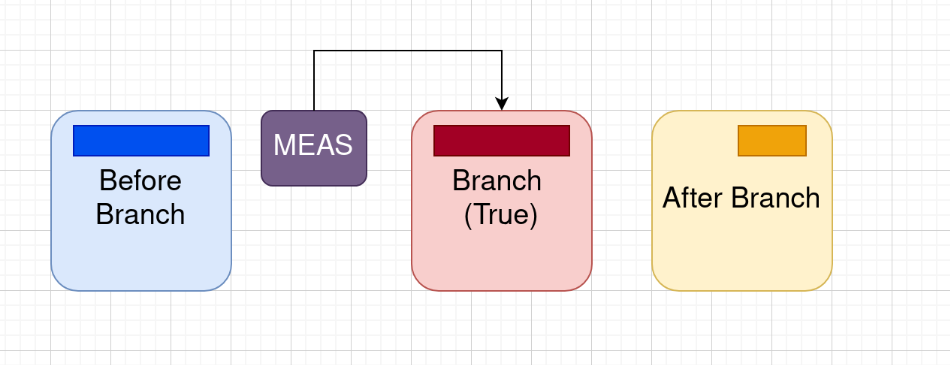
\includegraphics[width=0.8\textwidth]{Images/start.png}
    \caption{The General Setting}
  \end{figure}
\end{frame}

\begin{frame}{Split}
  \begin{figure}
    \centering
    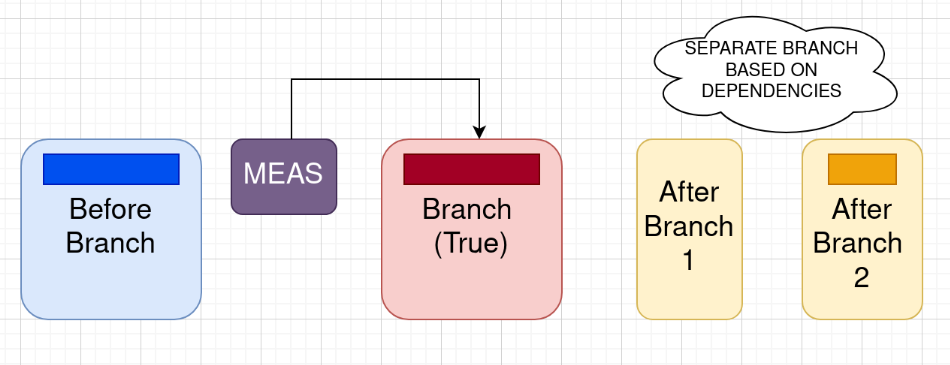
\includegraphics[width=0.8\textwidth]{Images/sep.png}
    \caption{Splitting the Branches}
  \end{figure}
\end{frame}

\begin{frame}{Recombine}
  \begin{figure}
    \centering
    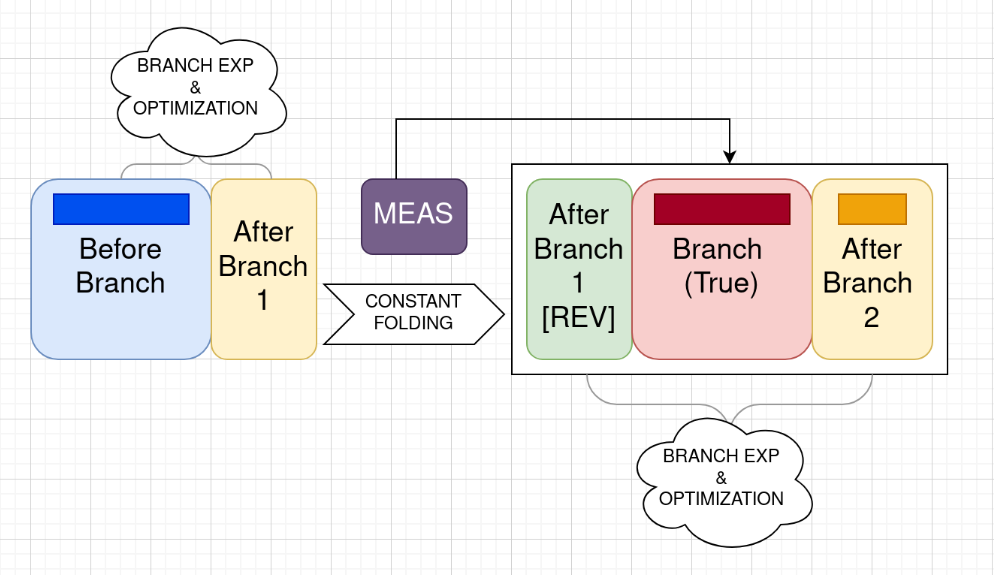
\includegraphics[width=0.8\textwidth]{Images/recomb.png}
    \caption{Recombining the Branches}
  \end{figure}
\end{frame}

\begin{frame}{The Issues}
  \begin{itemize}
    \item Measurements are the only \emph{non-commutative} operations in quantum circuits. Consequently, one cannot change the order of operations on measured quantum registers.
    \item Multiple branches are tougher to deal with as we are restricted to the non-dependent (wrt the measured registers) gates and registers. (Although this can be addressed to some extent later)
    \item Certain cases are easily dealt with in a nested fashion, while some are better flattened out (and some cannot be optimized at all).
    \item The extent of optimization is also dependent on the circuit area, level of nesting and window-depth.
  \end{itemize}
\end{frame}

\begin{frame}{A Toy Example}
  \begin{figure}
    \centering
    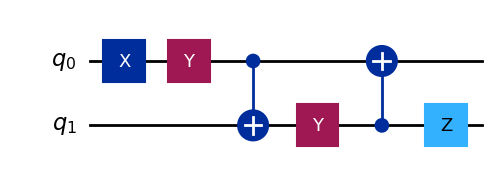
\includegraphics[width=0.8\textwidth]{Images/cond.png}
    \caption{A Toy Condition Subcircuit}
  \end{figure}
\end{frame}

\begin{frame}{The Toy Example}
  \begin{figure}
    \centering
    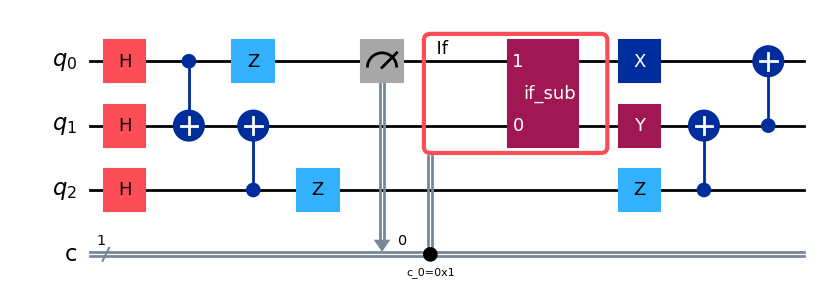
\includegraphics[width=0.8\textwidth]{Images/toy1.png}
    \caption{Without Optimization}
  \end{figure}

  \begin{block}{Analysis}
    \begin{itemize}
      \item \textbf{Gate Count:} RZ:7, SX:4, CX:3, X:2, IF\_ELSE:1
      \item \textbf{Depth:} 10
    \end{itemize}
  \end{block}
\end{frame}

\begin{frame}{The Toy Example}
  \begin{figure}
    \centering
    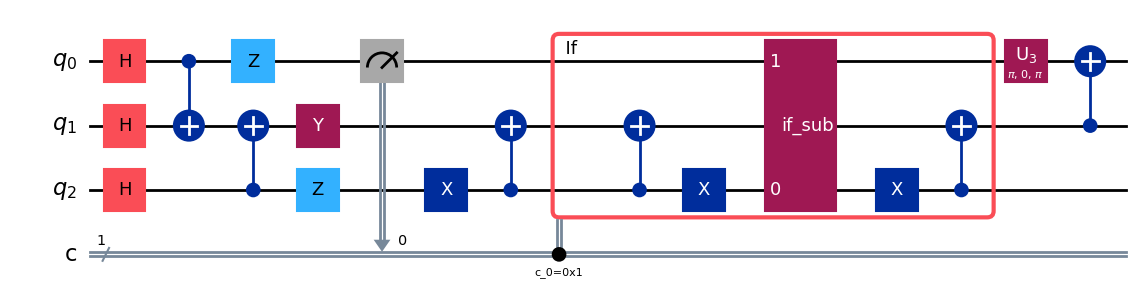
\includegraphics[width=0.8\textwidth]{Images/toy2.png}
    \caption{With Optimization}
  \end{figure}

  \begin{block}{Analysis}
    \begin{itemize}
      \item \textbf{Gate Count:} RZ:7, SX:3, CX:2, X:1, IF\_ELSE:1
      \item \textbf{Depth:} 7
    \end{itemize}
  \end{block}
\end{frame}

\begin{frame}{PseudoCode}
  \begin{figure}
    \centering
    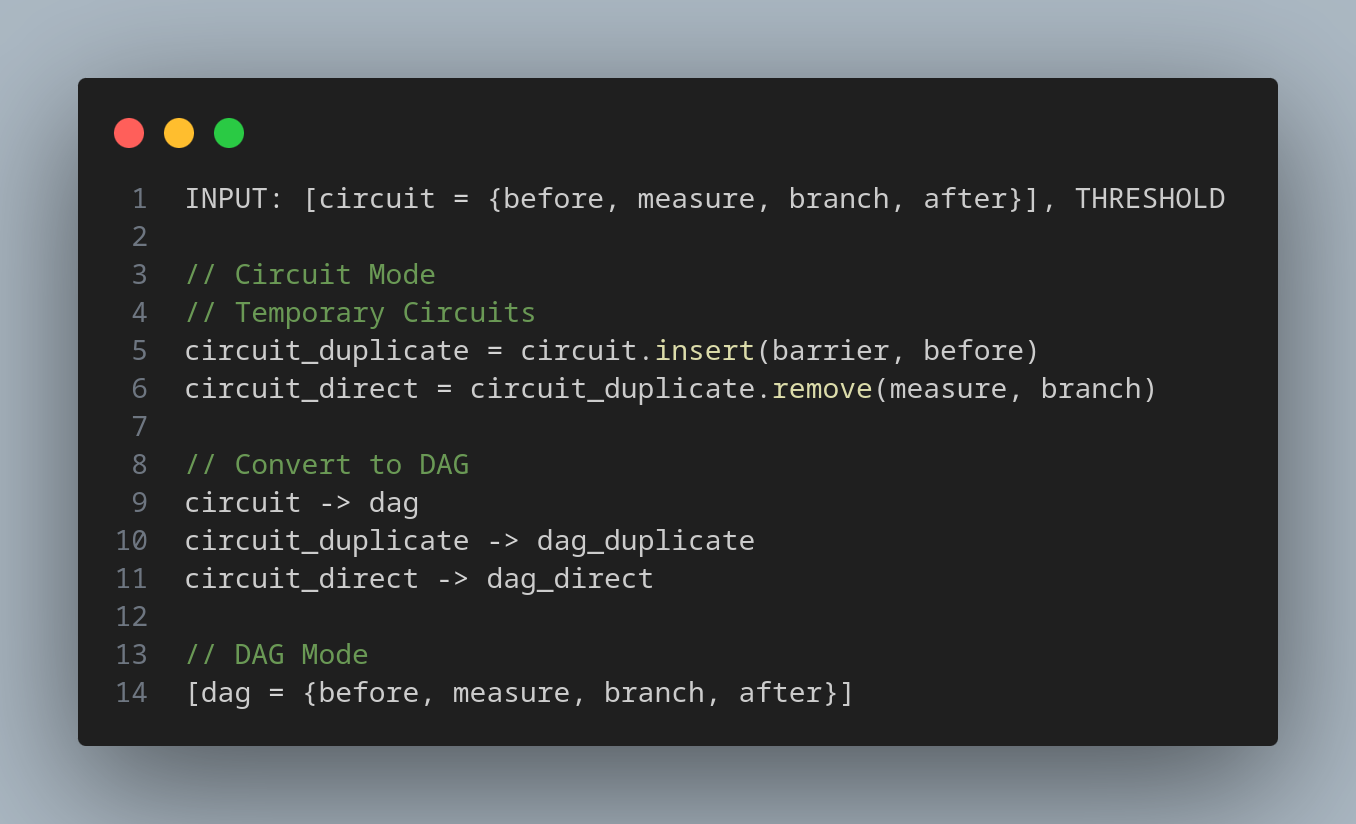
\includegraphics[width=0.8\textwidth]{Images/code_1.png}
    \caption{Alternate Circuit Generation}
  \end{figure}
\end{frame}

\begin{frame}{PseudoCode}
  \begin{figure}
    \centering
    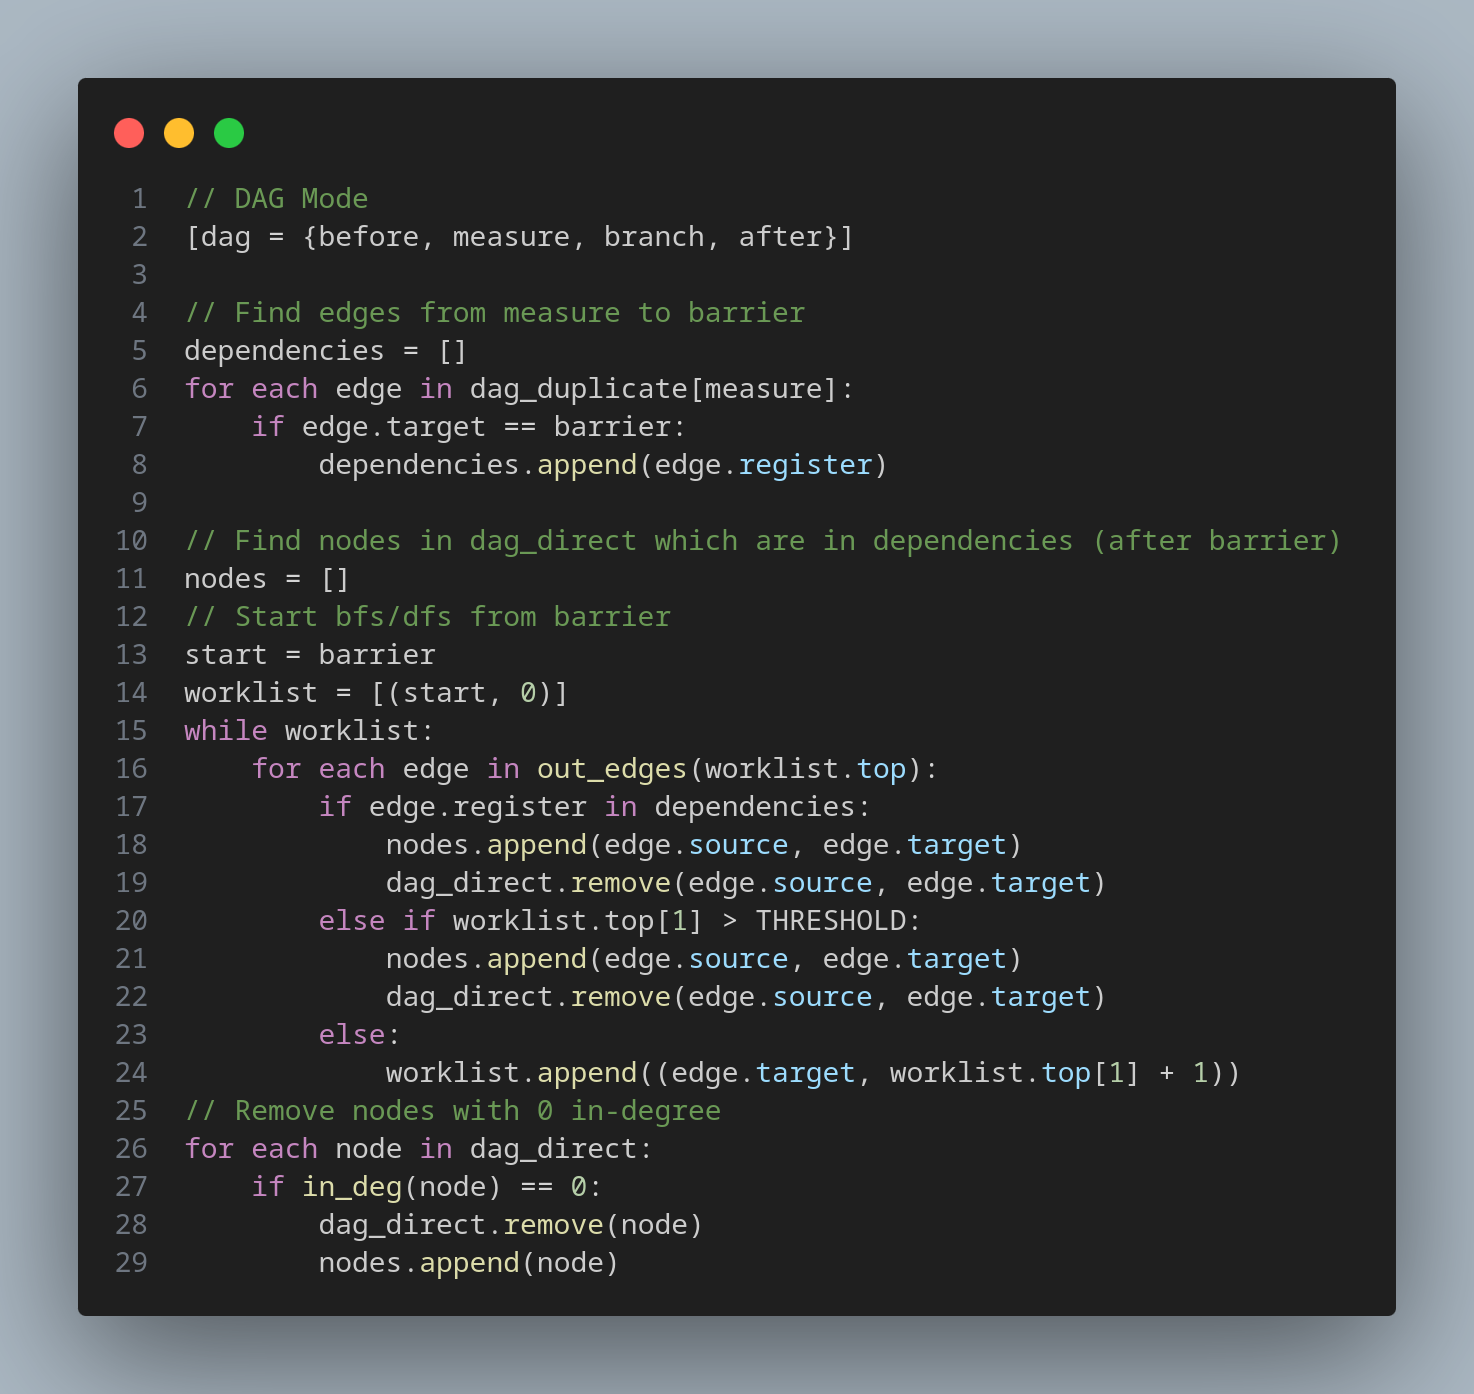
\includegraphics[width=0.8\textwidth]{Images/code_2.png}
    \caption{Idenitfy and Remove Dependencies}
  \end{figure}
\end{frame}

\begin{frame}{PseudoCode}
  \begin{figure}
    \centering
    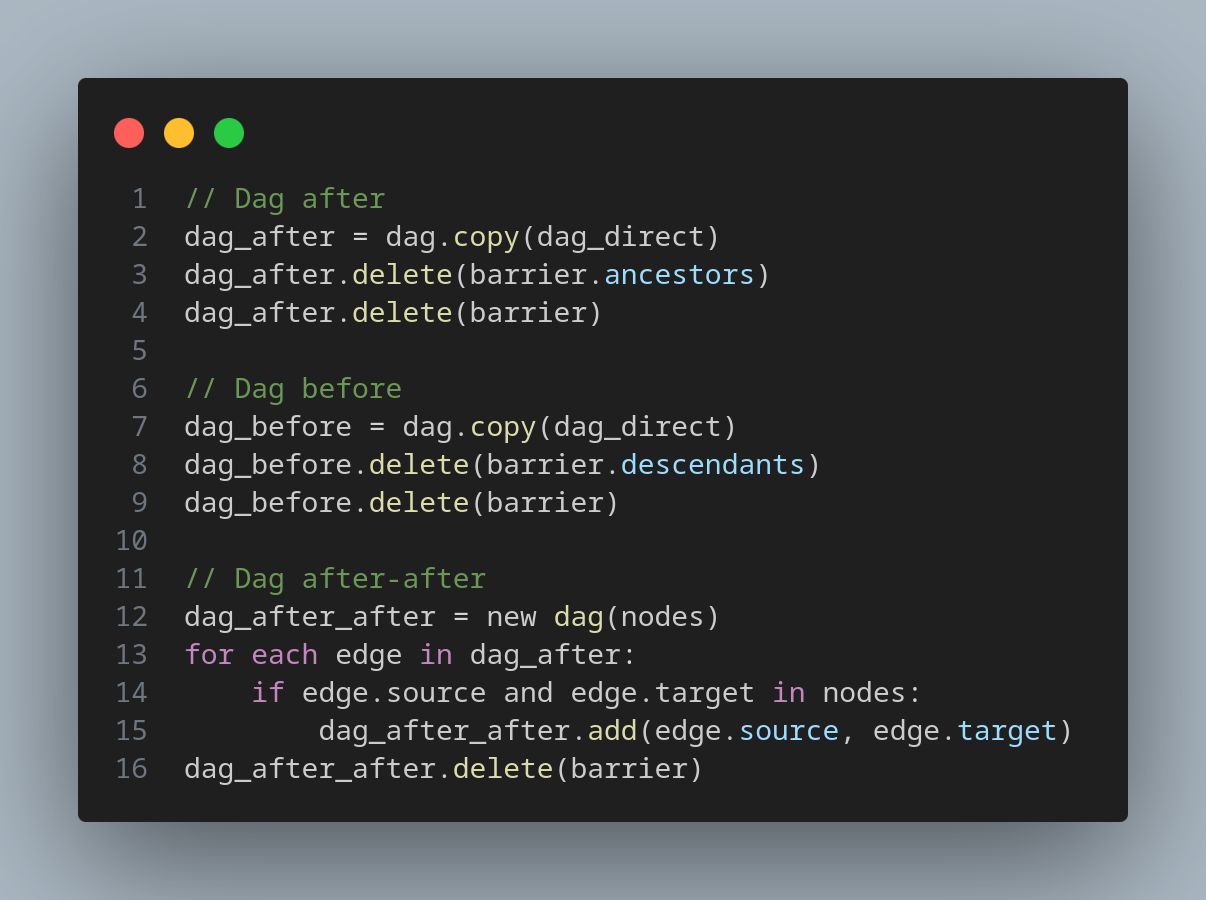
\includegraphics[width=0.8\textwidth]{Images/code_3.png}
    \caption{Convert DAGs to Sub-Circuits}
  \end{figure}
\end{frame}

\begin{frame}{PseudoCode}
  \begin{figure}
    \centering
    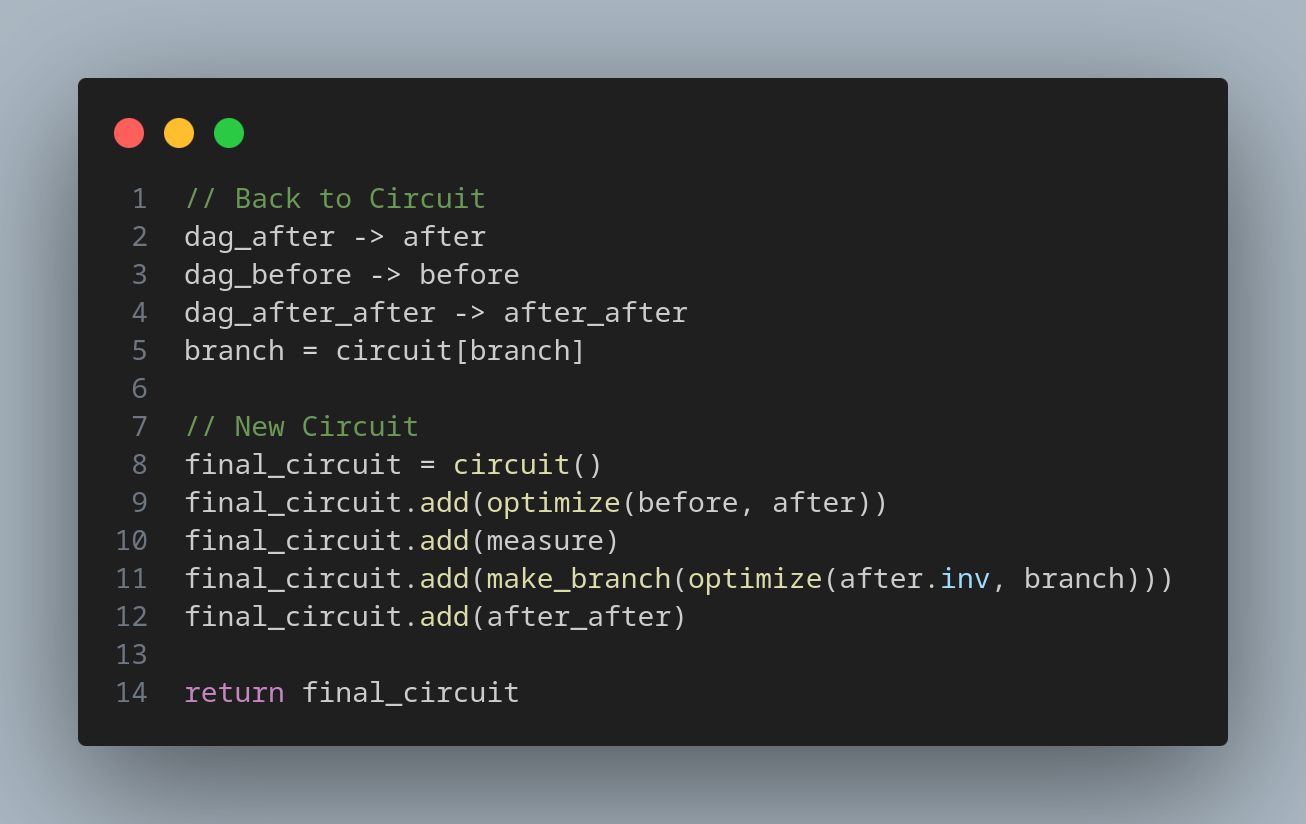
\includegraphics[width=0.8\textwidth]{Images/code_4.png}
    \caption{Finalize the Circuit}
  \end{figure}
\end{frame}

%%%%%%%%%%%%%%%%%%%%%%%%%%%%%%%%%%%%%%%%%%%%%%%%%%%%%%%%%%%%%%%%
\section{Hoare Optimizations++}
\begin{frame}{Hoare Optimizations++}
  \begin{itemize}
    \item Hoare Logic is a formal system using preconditions and postconditions to specify the behavior of a program.
    \item We can use Hoare Logic to optimize quantum circuits by ensuring that the optimizations do not change the correctness of the program.
    \item The following Hoare logic used could be state-dependent or state-independent.
  \end{itemize}
\end{frame}

%----------------------------------------------------------------
\begin{frame}{Example}
  \begin{figure}
    \centering
    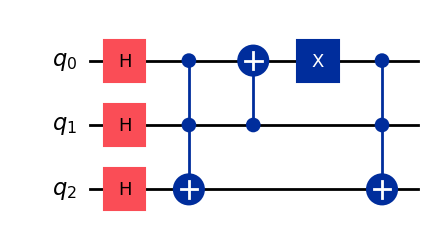
\includegraphics[width=0.5\textwidth]{Images/hoare_s1.png}
    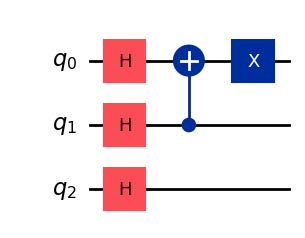
\includegraphics[width=0.4\textwidth]{Images/hoare_s2.png}
    \caption{Hoare Logic Example}
  \end{figure}
\end{frame}

%----------------------------------------------------------------

\begin{frame}{Works Across Measurements?}
  \begin{figure}
    \centering
    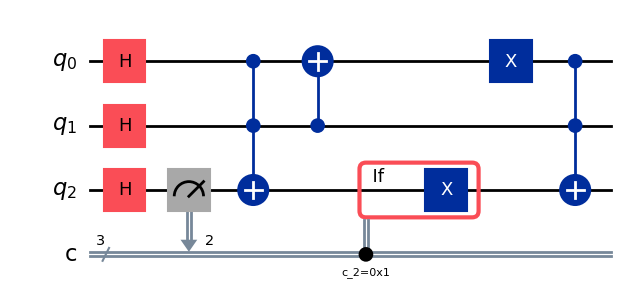
\includegraphics[width=0.5\textwidth]{Images/meas_1.png}
    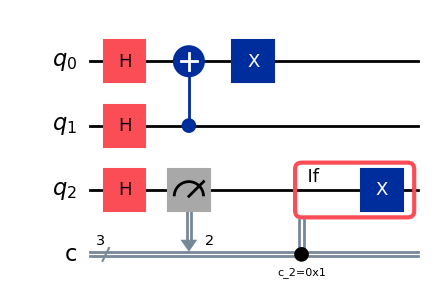
\includegraphics[width=0.4\textwidth]{Images/meas_2.png}
    \caption{Across Measurements}
  \end{figure}

  \begin{block}{Analysis}
    Original Circuit Gate Count: {'rz': 24, 'sx': 11, 'cx': 11, 'measure': 1, 'if\_else': 1}) \\
    Optimized Circuit Gate Count: {'rz': 6, 'sx': 3, 'cx': 1, 'x': 1, 'measure': 1, 'if\_else': 1})
  \end{block}
\end{frame}

%---------------------------------------------------------------

\begin{frame}{On Measurements}
  \begin{figure}
    \centering
    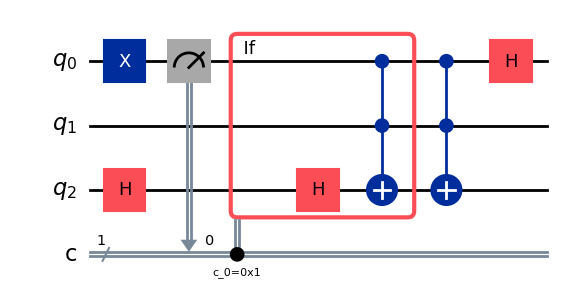
\includegraphics[width=0.4\textwidth]{Images/meas_3.png}
    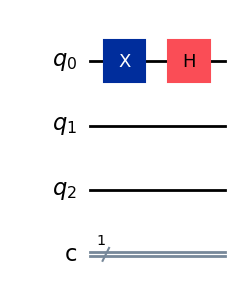
\includegraphics[width=0.25\textwidth]{Images/meas_4.png}
    \caption{On Measurements}
  \end{figure}

  \begin{block}{Analysis}
    Original Circuit Gate Count: {'rz': 13, 'cx': 6, 'sx': 4, 'x': 1, 'measure': 1, 'if\_else': 1} \\
    Optimized Circuit Gate Count: {'rz': 2, 'sx': 1}
  \end{block}
\end{frame}

%---------------------------------------------------------------

\begin{frame}{Value Independent}
  \begin{figure}
    \centering
    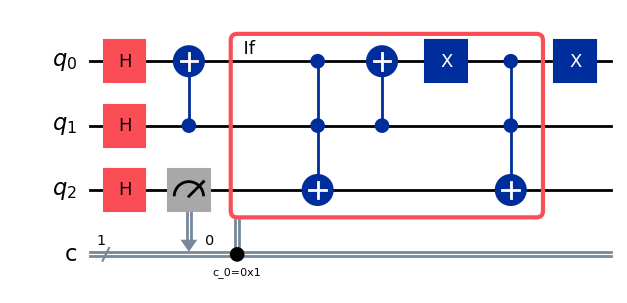
\includegraphics[width=0.4\textwidth]{Images/val_ind_1.png}
    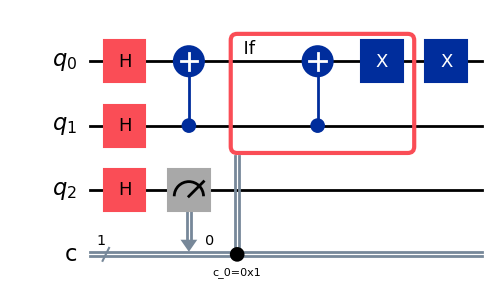
\includegraphics[width=0.4\textwidth]{Images/val_ind_2.png}
    \caption{Value Independent}
  \end{figure}

  \begin{block}{Analysis}
    Original Circuit Gate Count: {'rz': 6, 'sx': 3, 'cx': 1, 'measure': 1, 'if\_else': 1, 'x': 1} \\
    Optimized Circuit Gate Count: {'rz': 6, 'sx': 3, 'measure': 1, 'if\_else': 1}
  \end{block}
\end{frame}

%---------------------------------------------------------------
\begin{frame}{Value Dependent}
  \begin{figure}
    \centering
    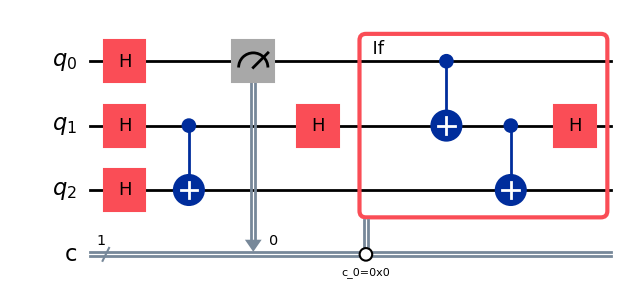
\includegraphics[width=0.4\textwidth]{Images/val_dep_1.png}
    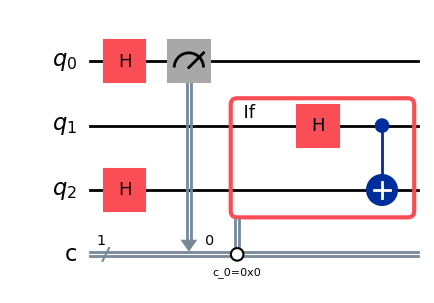
\includegraphics[width=0.4\textwidth]{Images/val_dep_2.png}
    \caption{Value Dependent}
  \end{figure}

  \begin{block}{Analysis}
    Original Circuit Gate Count: {'rz': 7, 'sx': 4, 'cx': 1, 'measure': 1, 'if\_else': 1} \\
    Optimized Circuit Gate Count: {'rz': 4, 'sx': 2, 'measure': 1, 'if\_else': 1}
  \end{block}
\end{frame}

%---------------------------------------------------------------
% Add your bibliography here
\begin{frame}[allowframebreaks]{References}
  \bibliographystyle{unsrt}
  \bibliography{ref}
\end{frame}

%---------------------------------------------------------------

\end{document}
